\subsection{Physikalischer Hintergrund}
\fbox{
	\parbox{\linewidth}{
		\textit{Ziel des Kapitels:}\\
		Anwendungsfall und Hintergrund vorstellen.\\[6px]
		\textit{Inhalte:}
		\begin{itemize}
		%	\setlength{\itemsep}{-5pt}
			\item Physikalischer Hintergrund
			\item Versuchsaufbau und Ablauf
		\end{itemize}
}}\\

Helmholtz-Spulen werden in der Physik an verschiedensten Stellen verwendet und spielen auch in der Ausbildung von Schülern und Studenten eine wichtige Rolle. Unter anderem werden sie in Schülerversuchen genutzt, um experimentell die Stärke des Erdmagnetfeldes zu bestimmen. Im Folgenden sollen die physikalischen Hintergründe kurz eingeführt sowie der Versuchsaufbau und -Ablauf erläutert werden.

\subsubsection{Spulen und Magnetfelder}
Wird eine elektrische Leiterschleife von einem Strom durchflossen, so induziert diese ein Magnetfeld. Dieses Feld verläuft sowohl durch das Innere als auch durch die Umgebung der Spule. Die Stärke des Feldes hängt dabei von der Windungszahl und dem Durchmesser der Spule sowie der angelegten Spannung ab.
Im Inneren der Spule ist das Magnetfeld \textit{homogen}. Das bedeutet, es ist an allen Punkten im Raum gleich ''stark'' und gleich gerichtet. Außerhalb der Spule hingegen ist das Feld \textit{inhomogen}, es erfüllt beide zuvor genannten Eigenschaften nicht.\\

Wie ''stark'' ein Magnetfeld an einer bestimmten Stelle ist, lässt sich dabei durch zwei Größen ausdrücken:
\begin{itemize}
	\setlength{\itemsep}{-5pt}
	\item Die\textit{ magnetische Feldstärke} $H$ in Ampere pro Meter
	\item Die \textit{magnetische Flussdichte} $B$ in Tesla (entspricht Volt mal Sekunde pro Quadratmeter)
\end{itemize}  
Beide hängen über eine Materialkonstante $\mu$ zusammen: $B = \mu \cdot H$. Die Konstante berücksichtigt die magnetischen Eigenschaften des Mediums, in dem sich das Feld befindet. Im Falle des vorliegenden Versuches handelt es sich dabei um Luft, die eine magnetische Permeabilität von ca. $\mu = 1 \cdot 4 \cdot 10^{-7}$ aufweist.\\

Im Weiteren meint diese Arbeit mit der ''Stärke'' des Magnetfeldes stets die magnetische Flussdichte in Tesla, es sei denn es ist entsprechend anders ausgewiesen.\\

\vspace{4px}
{\large\textit{Helmholtz-Spule}}\\
Bei einer Helmholtz-Spule handelt es sich im Prinzip um zum zwei zusammengeschaltete solcher Spulen. Dabei werden zwei identische Spulen nebeneinander aufgestellt und verbunden, sodass der Abstand genau dem Radius der Spulen entspricht. Abbildung \ref{img:Helmholtz} zeigt eine solche Helmholtz-Spule.\\

Durch diese spezielle Eigenschaft des Aufbaus überlagern sich die beiden, durch die einzelnen Spulen entstehenden Magnetfelder genau so, dass im Raum zwischen den Spulen ebenfalls ein homogenes Magnetfeld entsteht. Abbildung \ref{img:Magnetfeld-Helmholtzspule} zeichnet das Vektorfeld schematisch für die X-Z-Ebene ($Y=0$) in der Draufsicht von oben auf eine Helmholtz-Spule. Dabei ist zu erkennen, dass das Feld in weiten Teilen des durch die zwei Spulen aufgespannten Zylinders homogen ist. Lediglich am Rand und in unmittelbarer Nähe zu den Spulen wird das Feld zunehmend inhomogen.\\

Die magnetische Flussdichte einer Helmholtz-Spule im Mittelpunkt zwischen den Spulen vereinfacht sich zu folgender Gleichung:
\begin{equation}
	\label{eq:mfield}
	B = \mu_{0} \cdot \frac{8 \cdot I \cdot N}{\sqrt{125} \cdot R}
\end{equation}

Dabei entspricht $I$ der Stromstärke, $N$ der Anzahl Windungen, $R$ dem Radius und $\mu_{0}$ der magnetischen Permeabilität. Für andere Punkte im Raum lassen sich die Gleichungen im Allgemeinen nicht so vereinfachen und müssen numerisch gelöst werden.\\

\vspace{4px}
\textit{Darstellungsformen von Magnetfeldern}\\
Zur Visualisierung von Magnetfeldern haben sich zwei Darstellungsmodelle etabliert: Feldlinien und Vektoren. Beide stellen das Feld mit Richtung und Stärke im Raum dar, unterscheiden sich aber in der Art und Weise. Abbildung \ref{img:Magnetfeld-Helmholtzspule} zeigt eine gemeinsame Darstellung beider Ansätze für eine Helmholtz-Spule.\\

\textit{Das Feldlinienmodell}\\
Die Feldliniendarstellung ist wohl die häufiger anzutreffende Darstellungsform. Hier werden geschlossene, kontinuierliche Linien genutzt, um den magnetischen Fluss darzustellen. Die Richtung des Feldes an einem Punkt auf einer Feldlinie entspricht der Tangente an diesem Punkt und die Stärke des Feldes wird über den Abstand der Feldlinien dargestellt.\\

Diese Darstellung macht den Unterschied zwischen homogenen und inhomogenen Feldern besonders gut sichtbar, da bei einem homogenen Feld die Feldlinien parallel verlaufen, bei einem inhomogenen hingegen nicht. Außerdem ist die Darstellung über die Dichte der Feldlinien eng verbunden mit der magnetischen Flussdichte. Allerdings bedeutet diese Darstellungsform auch, dass je stärker das Feld ist, desto mehr Feldlinien auf gleichem Raum dargestellt werden müssen. Bei einer dreidimensionalen Darstellung steigt die Anzahl dabei quadratisch mit der Flussdichte.\\

\textit{Vektorfeld}\\
Im Gegensatz dazu wird in der Vektor-Darstellung das Feld über einzelne Vektoren repräsentiert. Dabei geben Richtung und Betrag eines Vektors den Feldstärkevektor des Magnetfeldes für genau einen Punkt an. So lässt sich die Feldstärke an einem durch einen Vektor repräsentierten Punkt im Raum direkt ablesen. Wo ein Feld homogen ist lässt sich jedoch nur durch das Vergleichen von mehreren Vektoren in Länge und Richtung feststellen. Dieses Modell hat gegenüber dem Feldlinienmodell jedoch den Vorteil, dass mit zunehmender Feldstärke nur die Vektoren länger werden, die Anzahl jedoch gleich bleiben kann.
	
\begin{figure}[h!]
	\centering
	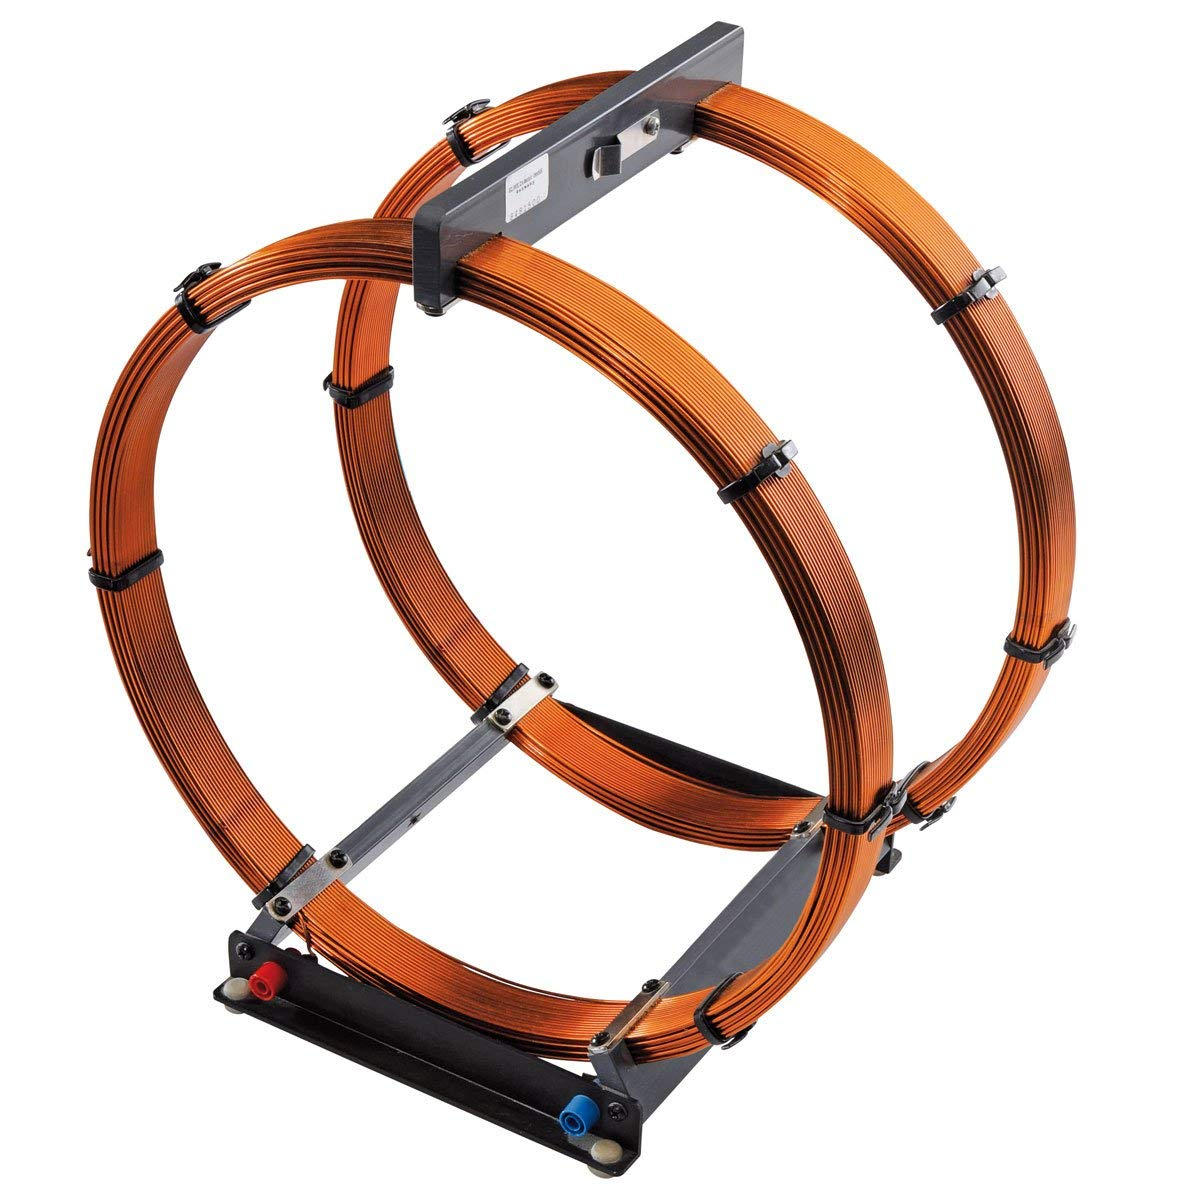
\includegraphics[width=0.45\textwidth]{images/Helmholtz.jpg}
	\caption{HH Spule}
	\label{img:Helmholtz}
\end{figure}

\begin{figure}[h!]
	\centering
	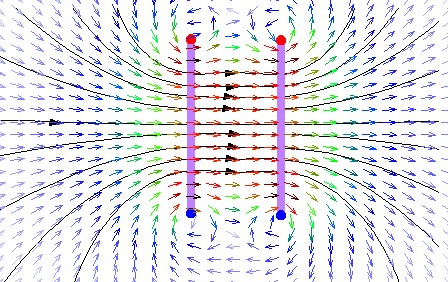
\includegraphics[width=0.65\textwidth]{images/Magnetfeld-Helmholtzspule.jpg}
	\caption{HH Spule MFeld Wikipedia}
	\label{img:Magnetfeld-Helmholtzspule}
\end{figure}

\subsubsection{Versuchsaufbau und Ablauf}
Ziel des Versuches ist die Bestimmung des Erdmagnetfeldes. Genauer bedeutet das die experimentelle Bestimmung von Richtung und magnetische Flussdichte des Feldes. Die Richtung kann dabei allein über den Kompass bestimmt werden. Die Flussdichte wird aus der gemessenen Stromstärke ermittelt, bei der die Helmholtz-Spule ein gleich starkes, eigenes Magnetfeld erzeugt.\\

\textit{Aufbau}\\
Der Versuchsaufbau ist in Abb. X skizziert und besteht aus: 
\begin{itemize}
%	\setlength{\itemsep}{-5pt}
	\item Einer Helmholtz-Spule mit fester Windungszahl und festem Radius
	\item Einem Kompass
	\item Einem in Reihe geschalteten Amperemeter
	\item Einer angeschlossenen Spannungsquelle
\end{itemize}

\textit{Ablauf}\\
Der Versuch läuft in zwei Teilen ab. Zunächst wird die Ausrichtung des Erdmagnetfeldes bestimmt und im nächsten Schritt dann die Flussdichte. Der Ablauf lässt sich wie folgt zusammenfassen:
\begin{enumerate}
	\setlength{\itemsep}{-2pt}
	\item Kompassnadel nach Norden ausrichten lassen
	\item Helmholtz-Spule orthogonal zur Kompassnadel ausrichten
	\item Spannungsquelle einschalten und Spannung langsam erhöhen
	\item Spannung erhöhen, bis Kompassnadel um 45° ausgelenkt ist
	\item Stromstärke ablesen und in Gleichung \eqref{eq:mfield} einsetzen
\end{enumerate}

Durch dieses Vorgehen wird im zweiten Schritt durch die Spule ein Magnetfeld erzeugt, das orthogonal zu dem der Erde gerichtet ist. Beide Felder überlagern sich, so dass sie den Kompass genau dann gleichmäßig in beide Richtungen auslenken, wenn beide Felder gleich stark auf die Nadel wirken.